\documentclass[12pt,a4paper]{article}

% Margins.
\setlength{\oddsidemargin}{0in}
\setlength{\evensidemargin}{0in}
\setlength{\headheight}{12pt}
\setlength{\headsep}{42pt}
\setlength{\topmargin}{-54pt}
\setlength{\textwidth}{6.5in}
\setlength{\textheight}{10in}

\usepackage{amsmath}
\usepackage{float}
\usepackage{graphicx}
\usepackage[hyphens]{url}
\usepackage{hyperref}	% Clickable links to figures, references and urls.
\usepackage{datetime}
\usepackage{subfigure}

% Links direct to top of figures.
\usepackage[all]{hypcap}

% Drawing.
\usepackage{pgf}
\usepackage{tikz}

% Listings for formatting code.
\usepackage{listings}
\usepackage{textcomp}
% General options.
\lstset{breaklines=true, basicstyle=\small\ttfamily, tabsize=4, numbers=left, stepnumber=1, frame=single, showstringspaces=false, upquote=true}
% C++ specific high-lighting. Comments are 50/50 shades of green/black and strings coloured with 60/40 red/black mixture.
\lstset{language=[ISO]C++, commentstyle=\color{green!50!black}, keywordstyle=\color{blue}, stringstyle=\color{red!60!black}}

%opening
\title{\vspace{-3cm}Physics for Engineers\\Assignment 06\\Electric Potential\\ Magnetic Force on Moving Charge and Biot--Savart Law}
\author{Attique Dawood}
\date{April 14, 2013\\Due: April 21, 2014\\[0.2cm] Last Modified: \today, \currenttime}
\begin{document}
\maketitle
\noindent\textbf{Question 1:} Solve Sessional - II.
\section{Electric Potential}
\noindent\textbf{Question 2:} A 1 C charge is located at origin.
\begin{itemize}
\item[a.] Find electric potential, $V_A$ at point A(-1, 3, 7).
\item[b.] Find electric potential, $V_B$ at point B(2, 1, -5).
\item[c.] Calculate the potential difference $V_{AB}$ between A and B.
\item[d.] Calculate the work done in moving a 2 C charge from A to B.
\end{itemize}
\noindent\textbf{Question 3:} A 2 C charge is located at (-3, 0, 2) and a -4 C charge is located at (2, -1, 9).
\begin{itemize}
\item[a.] Find electric potential at point A(1, 1, 0).
\item[b.] Find electric potential at point B(3, 1, 2).
\end{itemize}
\noindent\textbf{Question 4:} Point charges $q_1=2$ C, $q_2=-1$ C and $q_3=3$ C are located at (-2, 4, 1), (1, -5, -2) and (-2, 0, 7), respectively. Find the total work done in assembling these charges, assuming they are brought from infinity. Also find electric potential at origin.\\[0.2cm]
\section{Miscellaneous Problems}
\noindent\textbf{Question 5:} A 1 C charged particle moving with uniform velocity $\textbf{v}=3\hat y$ m/s enters a uniform magnetic field $\textbf{B}=10\hat z$ Wb/m$^2$. Calculate magnetic force on it.\\[0.2cm]
\noindent\textbf{Question 6:} An electron moves with uniform velocity $\textbf{v}=8\times 10^6\hat x$ m/s in a uniform magnetic field. If magnetic field (\textbf{B}) of magnitude 0.025 Wb/m$^2$ is perpendicular to $z$--axis and makes an angle of $60^0$ with $x$--axis then find the force on electron.\\[0.2cm]
\noindent\textbf{Question 7 \cite[Example 7.3, page 270]{Sadiku}:} A circular loop located on $x^2+y^2=9$, $z=0$ carries a direct current of 10 A along $\hat\phi$. Determine \textbf{H} at (0, 0, 4) and (0, 0, -4).\\[0.2cm]
\noindent\textbf{Question 8 \cite[PE 7.3, page 271]{Sadiku}:} A thin ring of radius 5 cm is placed on plane $z=1$ cm so that its centre is at (0, 0, 1 cm). If the ring carries 50 mA along $\hat\phi$, find \textbf{H} at
\begin{itemize}
\item[a.] (0 ,0, -l cm)
\item[b.] (0 ,0, 10 cm)
\end{itemize}
\noindent\textbf{Question 9 \cite[Example 7.1, page 266]{Sadiku}:} Find \textbf{H} at (0, 0, 5) due to triangular loop shown in figure \ref{Conducting-triangular-loop}.\\
\textbf{Answer: }$\textbf{H}=\textbf{H}_1+\textbf{H}_2+\textbf{H}_3=(-59.1\hat y)+(27.4\hat x+27.4\hat y+10.9\hat z)+(-30.6\hat x+30.6\hat y)$ mA/m.
\begin{figure}[H]
\centering
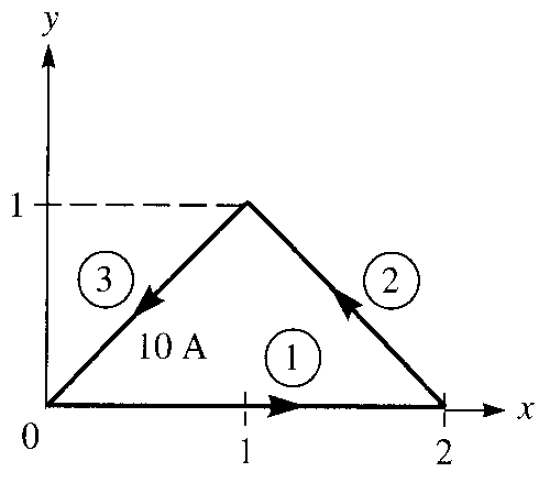
\includegraphics[scale=0.45]{Figure7-6aS.png}
\caption{Conducting triangular loop.}
\label{Conducting-triangular-loop}
\end{figure}
\newpage
\noindent\textbf{Question 10 \cite[Example 7.1, page 266]{Sadiku}:} Find \textbf{H} at (-3, 4, 0) due to semi--infinite current wires shown in figure \ref{Semi-infinite-wires}.\\
\textbf{Answer: }$\textbf{H}=\textbf{H}_z+\textbf{H}_x=(38.2\hat x+28.65\hat y)+23.88\hat z$ mA/m.
\begin{figure}[H]
\centering
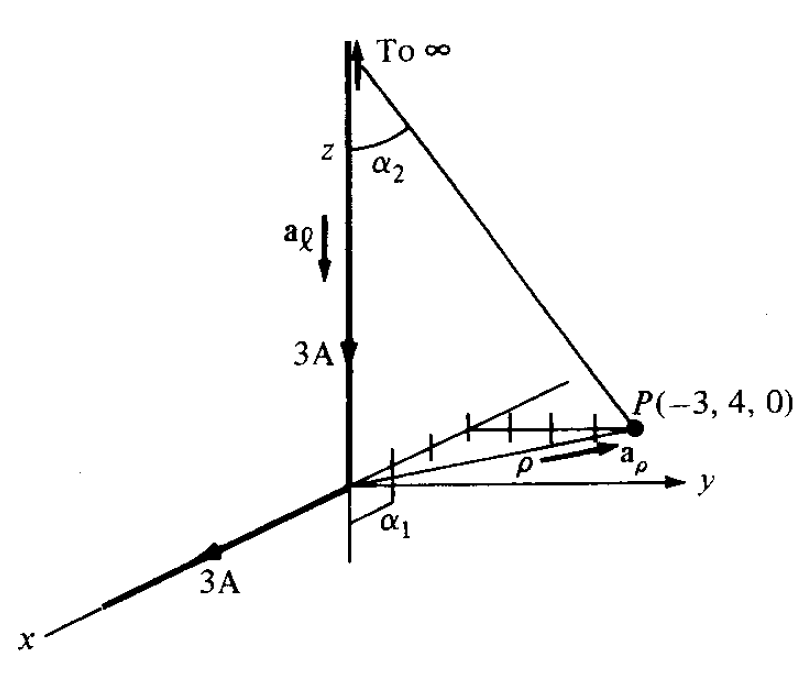
\includegraphics[scale=0.45]{Figure7-7aS.png}
\caption{Semi--infinite wires.}
\label{Semi-infinite-wires}
\end{figure}
\noindent\textbf{Question 11 \cite[Problem 7.3 and 7.4, page 297]{Sadiku}:} Find \textbf{H} at origin due to segment AB shown in figures \ref{AB-segment1} and \ref{AB-segment2}.\\
\begin{figure}[H]
\centering
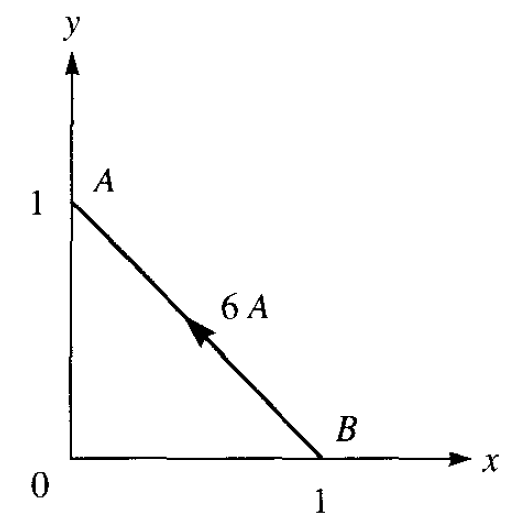
\includegraphics[scale=0.45]{Figure7-26S.png}
\caption{Current segment.}
\label{AB-segment1}
\end{figure}
\begin{figure}[H]
\centering
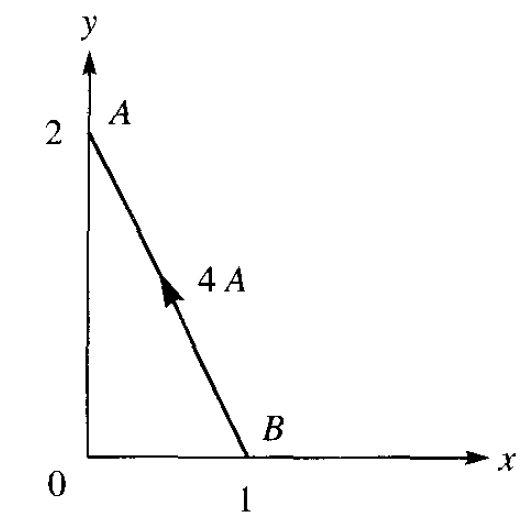
\includegraphics[scale=0.45]{Figure7-27S.png}
\caption{Current segment.}
\label{AB-segment2}
\end{figure}
\noindent\textbf{Question 12 \cite[Problem 7.8, page 298]{Sadiku}:} Find \textbf{H} at C due to current carrying loop forming an equilateral triangle shown in figure \ref{equilateral-wires}.\\
\begin{figure}[H]
\centering
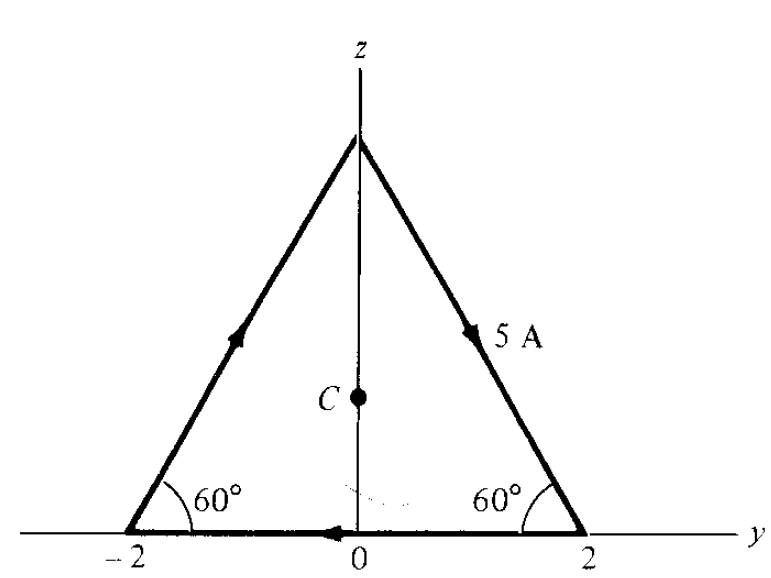
\includegraphics[scale=0.4]{Figure7-29S.png}
\caption{Loop forming equilateral triangle.}
\label{equilateral-wires}
\end{figure}
\noindent\textbf{Question 13 \cite[Problem 7.9, page 298]{Sadiku}:} Evaluate \textbf{H} at following points due to current loop shown in figure \ref{rectangular-loop}.
\begin{itemize}
\item[a.] (2, 2, 0)
\item[b.] (4, 2, 0)
\item[c.] (4, 8, 0)
\item[d.] (0, 0, 2)
\end{itemize}
\begin{figure}[H]
\centering
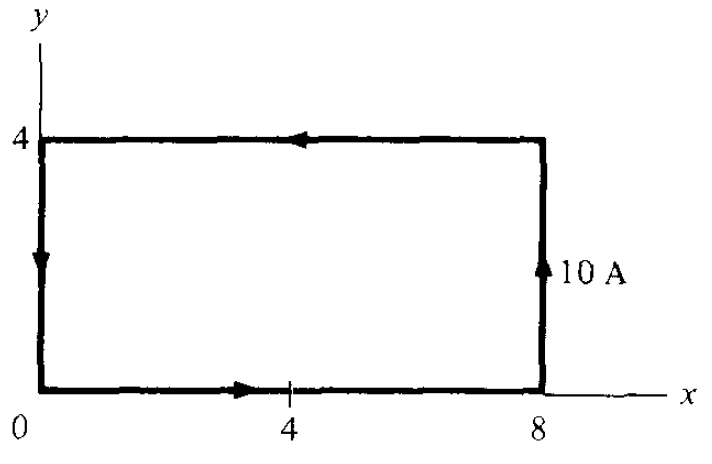
\includegraphics[scale=0.4]{Figure7-30S.png}
\caption{Rectangular loop.}
\label{rectangular-loop}
\end{figure}
\noindent\textbf{Question 14 \cite[Problem 7.9, page 298]{Sadiku}:} Evaluate \textbf{H} at origin due to current loop shown in figure \ref{semi-rectangular-loop}.\\
\begin{figure}[H]
\centering
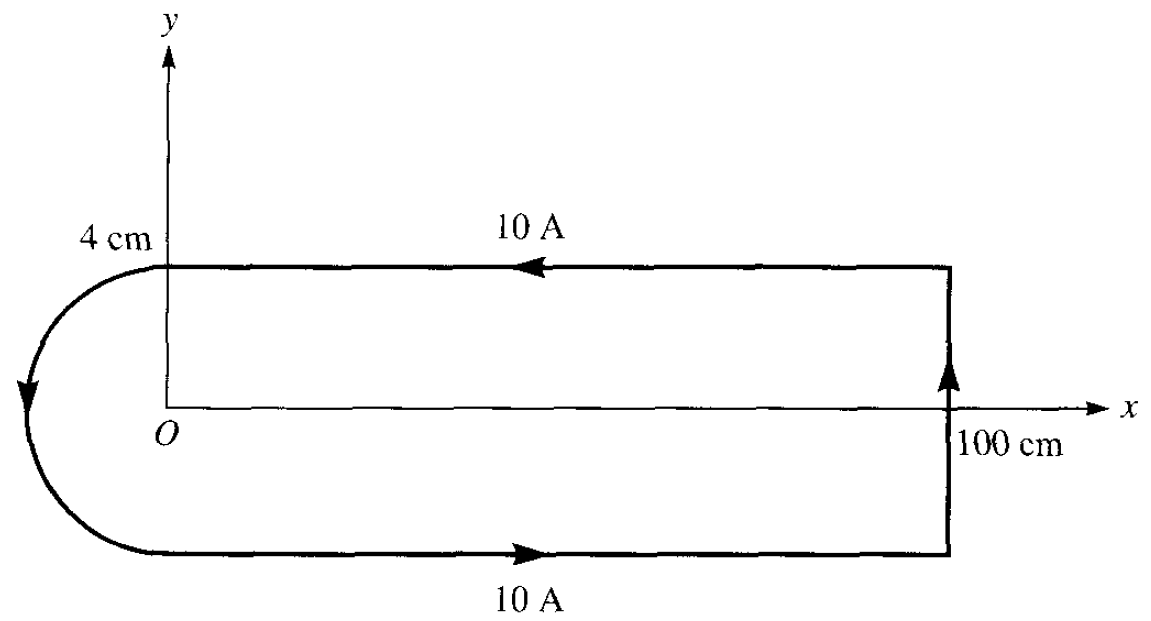
\includegraphics[scale=0.4]{Figure7-31S.png}
\caption{Current loop.}
\label{semi-rectangular-loop}
\end{figure}
\section{Problems from Text Books}
Solve the following end--of--chapter problems from Sadiku \cite[Ch. 7, pg. 296--297]{Sadiku}: 7.1b, 7.5, 7.7.
\section{Useful Formulas}
\subsection{Magnetic Field Due to a Finite Current--Carrying Segment of Wire}
\begin{equation}
\textbf{H}=\dfrac{I}{4\pi\rho}(\cos\alpha_2-\cos\alpha_1)\hat\phi.
\end{equation}
A conceptually simpler but mathematically intensive equivalent is
\begin{equation}
\textbf{H}=\dfrac{Ir_{12}}{4\pi|(\textbf{r}-\textbf{r}_1)\times\textbf{r}_{12}|}\left(\dfrac{(\textbf{r}-\textbf{r}_2)\cdot\textbf{r}_{12}}{|\textbf{r}-\textbf{r}_2|r_{12}}-\dfrac{(\textbf{r}-\textbf{r}_1)\cdot\textbf{r}_{12}}{|\textbf{r}-\textbf{r}_1|r_{12}}\right)\dfrac{(\textbf{r}-\textbf{r}_1)\times\textbf{r}_{12}}{|(\textbf{r}-\textbf{r}_1)\times \textbf{r}_{12}|}.
\end{equation}
Here \textbf{r} is the observation point, $\textbf{r}_1$ and $\textbf{r}_2$ are end points of wire such that current is flowing from $\textbf{r}_1$ to $\textbf{r}_2$.

A Matlab script is provided with this assignment based on the above formula. You can use it to check your answers. Follow following steps to run the script.
\begin{enumerate}
\item Open the \verb|HCurrentSegment.m| file by double--clicking on it. It should open in Matlab.
\item Set $\textbf{r}$, $\textbf{r}_1$, $\textbf{r}_2$ and $I$.
\item Press \verb|F5| or click on the button with green arrow that says \verb|Run|.
\item If you get a dialogue box asking whether to include or change Matlab path, select \verb|`Change Directory'| or \verb|`Add to Path'|.
\end{enumerate}

If one end of the wire is at infinity then take a very large number to represent the distance in Matlab, for example, if $\textbf{r}_1$ lies on $x$--axis at infinity then you can assign \verb|r1=[1e100 0 0];|. $1e100=1\times 10^{100}$.
\subsection{Infinite Current Carrying Wire}
Assuming wire is placed along $z$--axis and direction of current is along $\hat z$
\begin{equation}
\textbf{H}=\dfrac{I}{2\pi\rho}\hat\phi
\end{equation}
$\rho$ is perpendicular distance from wire to observation point and $\hat\phi$ is counter--clockwise direction following right hand rule with respect to current flow.
\subsection{Magnetic Field Due to a Current--Carrying Ring}
Magnetic field at the centre of a current carrying loop placed in $xy$--plane and centred at $z$--axis is given by $\textbf{H}=\dfrac{I}{4\pi\rho^2}(2\pi\rho)\hat z$. In case of a semi--circle or a wire shaped like an arc the magnetic field at centre is $\textbf{H}=\dfrac{I}{4\pi\rho^2}(\mathrm{arc~length})\hat z$. $\hat z$ direction assumes current is flowing counter--clockwise in $\hat\phi$ direction.
\bibliographystyle{plain}
\bibliography{PhysicsRef}
\end{document}
